\chapter{Dual Ascent}\label{ch:dualascent}

The dual ascent algorithm is the dual version for the problem of the minimum
\emph{Steiner} tree, which tries to find a directed subtree that connects a root
node to a selected subset of existing nodes called \emph{target} nodes. While in
the Steiner tree the purpose is to minimize the total cost of the links used in
the resulting broadcast tree, in the dual ascent version the goal is to maximize
the flow, which is flowing from node 1 to all other nodes. Both versions find
the same lower bound for the optimal solution, according to the mathematical
definition of a dual problem.

The minimum Steiner tree problem is defined as in \eqref{eq:primalproblem}.

\begin{equation}\label{eq:primalproblem}
	\begin{cases}
		\min\sum\limits_{(i,j) \in E} c_{ij}y_{ij}\\[10pt]
		\sum\limits_{h \in N} x_{ih}^k - \sum\limits_{j \in N} x_{ji}^k
		=
		\begin{cases}
			1 & i = 1\\
			-1 & i = k\\
			0 & i \neq 1,k\\
		\end{cases}\\[10pt]
		x_{ij}^k \leq y_{ij}\\[10pt]
		x_{ij}^k \geq 0 \qquad \forall (i,j) \in E, \forall k \in
		V\\[10pt]
		y_{ij} \in \{0, 1\}
	\end{cases}
\end{equation}
%\begin{equation}\label{eq:primalproblem}
%	\begin{cases}
%		\min\sum\limits_{(i,j) \in E} c_{ij}y_{ij}\\
%		\sum\limits_{i \in N_1} \sum\limits_{j \in \overline{N_1}}
%		y_{ij} \geq 1 & \forall N_1 \subseteq N : 1 \in N_1\
%		\mathrm{and}\ N_1 \cap V \neq \emptyset\\
%		y_{ij} \in \{0, 1\}
%	\end{cases}
%\end{equation}

Where \(E\) is the set of links; \(c_{ij}\) are the costs of the complete graph
for the link that goes from the node i to the node j; \(y_{ij}\) is a binary
variable which tells if the arc (i, j) is taken into the solution; \(x_{ij}^k\)
is a variable represents the amount of flow between node 1 and node k that flows
on the (i, j) arc; \(N\) is the whole set of nodes; \(V\) is the set of target
nodes.

From linear programming, we can derive the dual of the problem in
\eqref{eq:primalproblem}. This is shown in \eqref{eq:dualproblem}.

\begin{equation}\label{eq:dualproblem}
	\begin{cases}
		\max\sum\limits_{k \in V} R_k^k\\[10pt]
		R_j^k - R_i^k - w_{ij}^k \leq 0 & k \in V\\[10pt]
		\sum\limits_{k \in V} w_{ij}^k \leq c_{ij} & (i, j) \in
		E\\[10pt]
		w_{ij}^k \geq 0
	\end{cases}
\end{equation}

Where \(R_i^k\) is the dual flow value computed as the flow that starts from
node 1 to node k passing through node i, selecting the node k as one of the root
component nodes (\(R_1^k\) is set to 0 because otherwise there is one redundant
equation) and \(w_{ij}^k\) is the maximum slack between the node i and the node
j. The slack value is initialized by computing the difference between the (i, j)
arc cost (\(c_{ij}\)) and the \(w_{ij}^k\) value, which is initialized to 0, so
it's the (i, j) arc cost. The slack value is updated in each algorithm's step by
decreasing it by the amount of slack on the arc with the minimum cost.

The dual ascent algorithm aims to solve the dual of the Steiner tree problem.

\section{Comparison with Dijkstra}\label{sec:comparison}

The Dijkstra algorithm tries to find a minimum \emph{spanning} tree which
contains links that connect a set of target nodes.

Differently from that, the minimum \emph{Steiner} tree considers for the
computations, to connect all the target nodes, also other nodes. So in this way
the lower bound of the optimal solution is less or equal than the result
provided by a \emph{spanning} tree algorithm (as we can see in
\figref{fig:steiner}). The price to pay is in term of time and computational
power, because the algorithm has to visit all the possible links and not the
subset that involves only the target nodes, so this solution has a limited
scalability.

\begin{figure}
	\centering
	\begin{subfigure}[b]{0.3\textwidth}
		\centering
		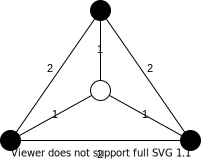
\includegraphics[width=\textwidth]{img/steiner-topology}
		\caption{An example of a network topology where black nodes are
		target nodes}\label{subfig:steiner-topology}
	\end{subfigure}
	\begin{subfigure}[b]{0.3\textwidth}
		\centering
		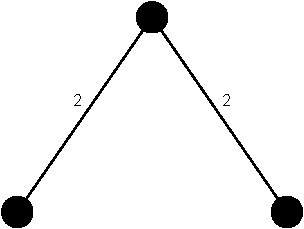
\includegraphics[width=\textwidth]{img/steiner-minspanning}
		\caption{The result of a minimum spanning tree algorithm on the
		example network topology. The result only contains links that
		involve target nodes. Its cost is
		4}\label{subfig:steiner-minspanning}
	\end{subfigure}
	\begin{subfigure}[b]{0.3\textwidth}
		\centering
		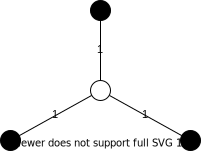
\includegraphics[width=\textwidth]{img/steiner-minsteiner}
		\caption{The result of a minimum Steiner tree algorithm on the
		example network topology. It includes also non-target nodes to
		build the tree. Its cost is 3}\label{subfig:steiner-minsteiner}
	\end{subfigure}
	\caption{An example of application of a minimum spanning tree algorithm
		and a minimum Steiner tree algorithm on the same
		topology}\label{fig:steiner}
\end{figure}


\section{The algorithm}\label{sec:algorithm}

The dual ascent algorithm starts from the root node and works
iteratively. There are three important data structures:

\begin{description}
	\item[Root Component] A set of strongly connected nodes, containing at
		least a target node, which hasn't incoming links from other
		target nodes or from the root node.
	\item[Auxiliary Graph] A graph which starts with all the topology nodes
		(including the non-target ones) and no links. At each iteration
		of the algorithm, the link with the minimum cost is added.
	\item[Reduced Cost Table] A table which stores the costs of connected
		nodes. Element \(R_i^j\) represents the dual cost to reach the
		node \(i\), selecting as root component the node \(j\). The
		final cost of the algorithm is the sum of all \(R_k^k\) values
		(slacks), where \(k\) is the index of a target node.
\end{description}

At each step a list of current root components is extracted from the auxiliary
graph. For each element of the list the algorithm finds, from the starting
topology, the link with minimum cost that has the root component as destination
and adds it to the auxiliary graph. Then the reduced cost table is updated by
decreasing the new cost value with the one that involved that node, selected at
the first iteration of the algorithm (the minimum one). The value obtained is
the \emph{slack}, that is added into \(R_j^j\) elements. Also values \(R_i^j\)
are updated considering the new paths formed in the auxiliary graph.

These steps are done until there are no remaining root components or no new
links from the starting topology. If in the auxiliary graph there are any
cycles, they are resolved deleting highest cost paths, so that the final result
is a broadcast tree including all the target nodes with zero or some non-target
ones.

